\documentclass[10pt,twocolumn]{article}

\usepackage[margin=0.75in]{geometry}
\usepackage{amsmath,amssymb,amsfonts}
\usepackage{graphicx}
\usepackage{booktabs}
\usepackage{hyperref}
\usepackage{xurl}
\usepackage{xcolor}
\usepackage{microtype}
\usepackage{cite}

\hypersetup{
    colorlinks=true,
    linkcolor=blue!70!black,
    citecolor=blue!70!black,
    urlcolor=blue!70!black
}

\title{\textbf{The Algorithmic Monoculture Paradox: Simulating the Collapse of Collective Intelligence in Foundation-Model-Mediated Social Networks}}

\author{
    \begin{tabular}[t]{c}
        \textbf{Ashuraj Santosh Herode}\textsuperscript{*} \\
        Department of Computer Engineering \\
        Vidyalankar Institute of Technology \\
        University of Mumbai, Mumbai, India \\
        \texttt{herodeashuraj@gmail.com}
    \end{tabular}
    \qquad\qquad
    \begin{tabular}[t]{c}
        \textbf{Dr. Prakash Parmar} \\
        Department of Computer Engineering \\
        Vidyalankar Institute of Technology \\
        University of Mumbai, Mumbai, India \\
        \texttt{prakash.parmar@vit.edu.in}
    \end{tabular}
}

\date{\today}

\begin{document}

\maketitle

\begin{abstract}
The ``Wisdom of Crowds'' principle demonstrates that distributed groups of imperfect decision-makers can achieve superior collective accuracy because independent, idiosyncratic errors cancel out upon aggregation. Today, the rapid integration of centralized foundation models (LLMs) into decision-making workflows threatens the epistemic independence that underlies this dynamic. When independent human agents query shared foundation models, individual error variance is suppressed, replacing independent noise with shared, correlated algorithmic bias. Here, we investigate this phenomenon by formalizing a discrete-event network simulation combining Scott Page's Diversity Prediction Theorem with a hybrid DeGroot consensus framework across macro-scale social graphs ($N = 1,000$ agents). Across 2,970 Monte Carlo simulations spanning three canonical network topologies (Watts-Strogatz Small-World, Barabási-Albert Scale-Free, and Erd\H{o}s-R\'enyi Random) and three correlation regimes, we show that high reliance on a centralized foundation model ($\rho = 0.90$) causes an 18- to 68-fold surge in Collective Squared Error (from $0.246$ to $16.833$), driven by the rapid collapse of cognitive diversity. Furthermore, we demonstrate that an oligopoly of competing foundation models ($\rho = 0.50$) fails to prevent this collapse (Collective Error surges to $10.314$), whereas an unconstrained polyculture ($\rho = 0.00$) preserves collective wisdom (Collective Error bounded at $3.974$). These findings prove that individual optimization under shared generative AI triggers systemic epistemic fragility, highlighting urgent implications for AI governance, platform auditing, and sociotechnical system design.
\end{abstract}

\section{Introduction}
For over a century, social epistemology and mathematical statistics have recognized that collective intelligence emerges from cognitive diversity \cite{galton1907vox, page2007difference}. In classical human deliberation, whether forecasting economic indices, evaluating scientific hypotheses, or curating public knowledge, individual human agents possess idiosyncratic biases and noisy heuristics. Crucially, when these errors are uncorrelated, aggregation mechanics—such as averaging or consensus formation—cause noise to cancel out, allowing the collective judgment of the crowd to outperform even its most capable individual members.

The rapid, worldwide deployment of generative foundation models (Large Language Models, or LLMs) has disrupted this epistemic architecture. Today, millions of professionals, researchers, students, and autonomous software agents rely on a small handful of centralized foundation models for heuristic guidance, text synthesis, and decision support. 

At the individual level, this technological transition is undeniably advantageous: querying an aligned foundation model reduces individual task completion time, resolves syntactical ambiguities, and frequently lowers individual error relative to uninformed guessing. However, evaluating AI assistance purely at the level of the individual decision-maker commits an ecological fallacy. As formalized by Kleinberg and Raghavan \cite{kleinberg2021algorithmic}, when independent entities adopt identical or highly correlated algorithmic decision rules, the system exhibits \textbf{Algorithmic Monoculture}.

Recent empirical audits have confirmed that aligned foundation models exhibit severe \textit{Generative Monoculture} \cite{bommasani2024generative}: due to alignment techniques such as Reinforcement Learning from Human Feedback (RLHF) and Direct Preference Optimization (DPO), models truncate output support, homogenizing stylistic variance and reinforcing centralized ideological priors. 

While existing literature has examined algorithmic monoculture in static, isolated classification tasks (such as credit scoring or resume screening) \cite{kleinberg2021algorithmic}, the sociotechnical reality of human discourse is fundamentally networked. Humans do not interact with algorithms in isolation; they deliberate, exchange beliefs, and form consensus across structured communication topologies \cite{watts1998collective, barabasi1999emergence, golub2010naive}.

This paper addresses a fundamental open question at the intersection of network science, social computing, and AI governance:
\begin{quote}
\textit{At what critical threshold of algorithmic reliance ($\alpha$) does a networked crowd transition from the ``Wisdom of Crowds'' into collective epistemic degradation, and does network topology buffer or accelerate this collapse?}
\end{quote}

Through a macro-scale computational framework encompassing 2,970 Monte Carlo simulations across $1,000$-agent networks, we formalize the interaction between Scott Page's Diversity Prediction Theorem \cite{page2007difference} and hybrid DeGroot consensus dynamics \cite{degroot1974reaching, golub2010naive}. Our findings demonstrate that algorithmic monoculture acts as an epistemic variance-destroyer, triggering non-linear surges in collective error even when individual models appear locally accurate.

\section{Theoretical Framework \& Related Work}

\subsection{The Diversity Prediction Theorem}
Let $\theta \in \mathbb{R}$ represent an objective ground truth parameter. Suppose a crowd of $n$ agents provides estimates $s_1, s_2, \dots, s_n$. The mean collective prediction is defined as $c = \frac{1}{n} \sum_{i=1}^n s_i$. 

Page \cite{page2007difference} established that collective squared error can be exactly decomposed into two opposing terms:
\begin{equation}
(c - \theta)^2 = \frac{1}{n} \sum_{i=1}^n (s_i - \theta)^2 - \frac{1}{n} \sum_{i=1}^n (s_i - c)^2
\label{eq:page_theorem}
\end{equation}
which is expressed conceptually as:
\begin{equation}
\mathrm{Error}_{\mathrm{coll}} = \overline{\mathrm{Error}}_{\mathrm{ind}} - \mathrm{Diversity}
\end{equation}

Equation \ref{eq:page_theorem} holds as an exact mathematical identity. Crucially, the minus sign demonstrates that cognitive diversity (the variance of individual estimates around the crowd mean) is not merely a social virtue, but a direct mathematical offset against collective error. If an algorithmic intervention reduces individual error by a modest margin but severely collapses cognitive diversity, the collective prediction must strictly degrade.

\subsection{Correlated Noise and Monoculture}
In classical crowds, individual estimates follow an independent noise model:
\begin{equation}
s_i = \theta + \epsilon_i, \quad \mathbb{E}[\epsilon_i] = 0, \quad \text{Cov}(\epsilon_i, \epsilon_j) = 0 \quad (\forall i \neq j)
\end{equation}
Under independent noise, the variance of the sample mean scales as $\text{Var}(c) = \frac{\sigma^2}{n} \xrightarrow{n \to \infty} 0$. 

Following Kleinberg and Raghavan \cite{kleinberg2021algorithmic}, we introduce an algorithmic foundation model providing advice $\hat{\theta}_M = \theta + \mu_{AI} + \eta$, where $\mu_{AI}$ is systemic bias and $\eta \sim \mathcal{N}(0, \sigma^2_{AI})$ is shared structural error. When agents rely on the model with weight $\alpha \in [0, 1]$, individual estimates become:
\begin{equation}
s_i(\alpha) = (1 - \alpha)(\theta + \epsilon_i) + \alpha(\theta + \mu_{AI} + \eta)
\end{equation}
As $n \to \infty$, the crowd mean converges to:
\begin{equation}
\lim_{n \to \infty} c(\alpha) = \theta + \alpha \mu_{AI} + \alpha \eta
\end{equation}
Because $\eta$ is shared identically across all querying nodes, $\text{Var}(c(\alpha)) = \alpha^2 \sigma^2_{AI} > 0$. The error cancellation property guaranteed by the Law of Large Numbers is destroyed.

\subsection{Network Epistemology \& Social Topologies}
Real-world deliberating crowds communicate across complex networks $G = (V, E)$ \cite{zollman2007communication}. Two structural properties dictate information propagation:
\begin{enumerate}
    \item \textbf{Watts-Strogatz Small-World Graphs:} Characterized by high clustering coefficients ($C \gg C_{\text{random}}$) and short average path lengths ($L \sim \ln N$), typical of dense professional disciplines and localized communities \cite{watts1998collective}.
    \item \textbf{Barab\'asi-Albert Scale-Free Graphs:} Generated via preferential attachment, yielding power-law degree distributions $P(k) \sim k^{-\gamma}$, where central hubs dominate communication cascades \cite{barabasi1999emergence}.
\end{enumerate}

\section{Model \& Simulation Methodology}

\subsection{Simulation Engine Architecture}
We model an epistemic community of $N = 1,000$ agents situated on a graph $G = (V, E)$ constructed using NetworkX \cite{hagberg2008exploring}. The simulation advances across discrete time steps $t \in \{0, 1, \dots, T\}$.

\begin{figure*}[t]
\centering
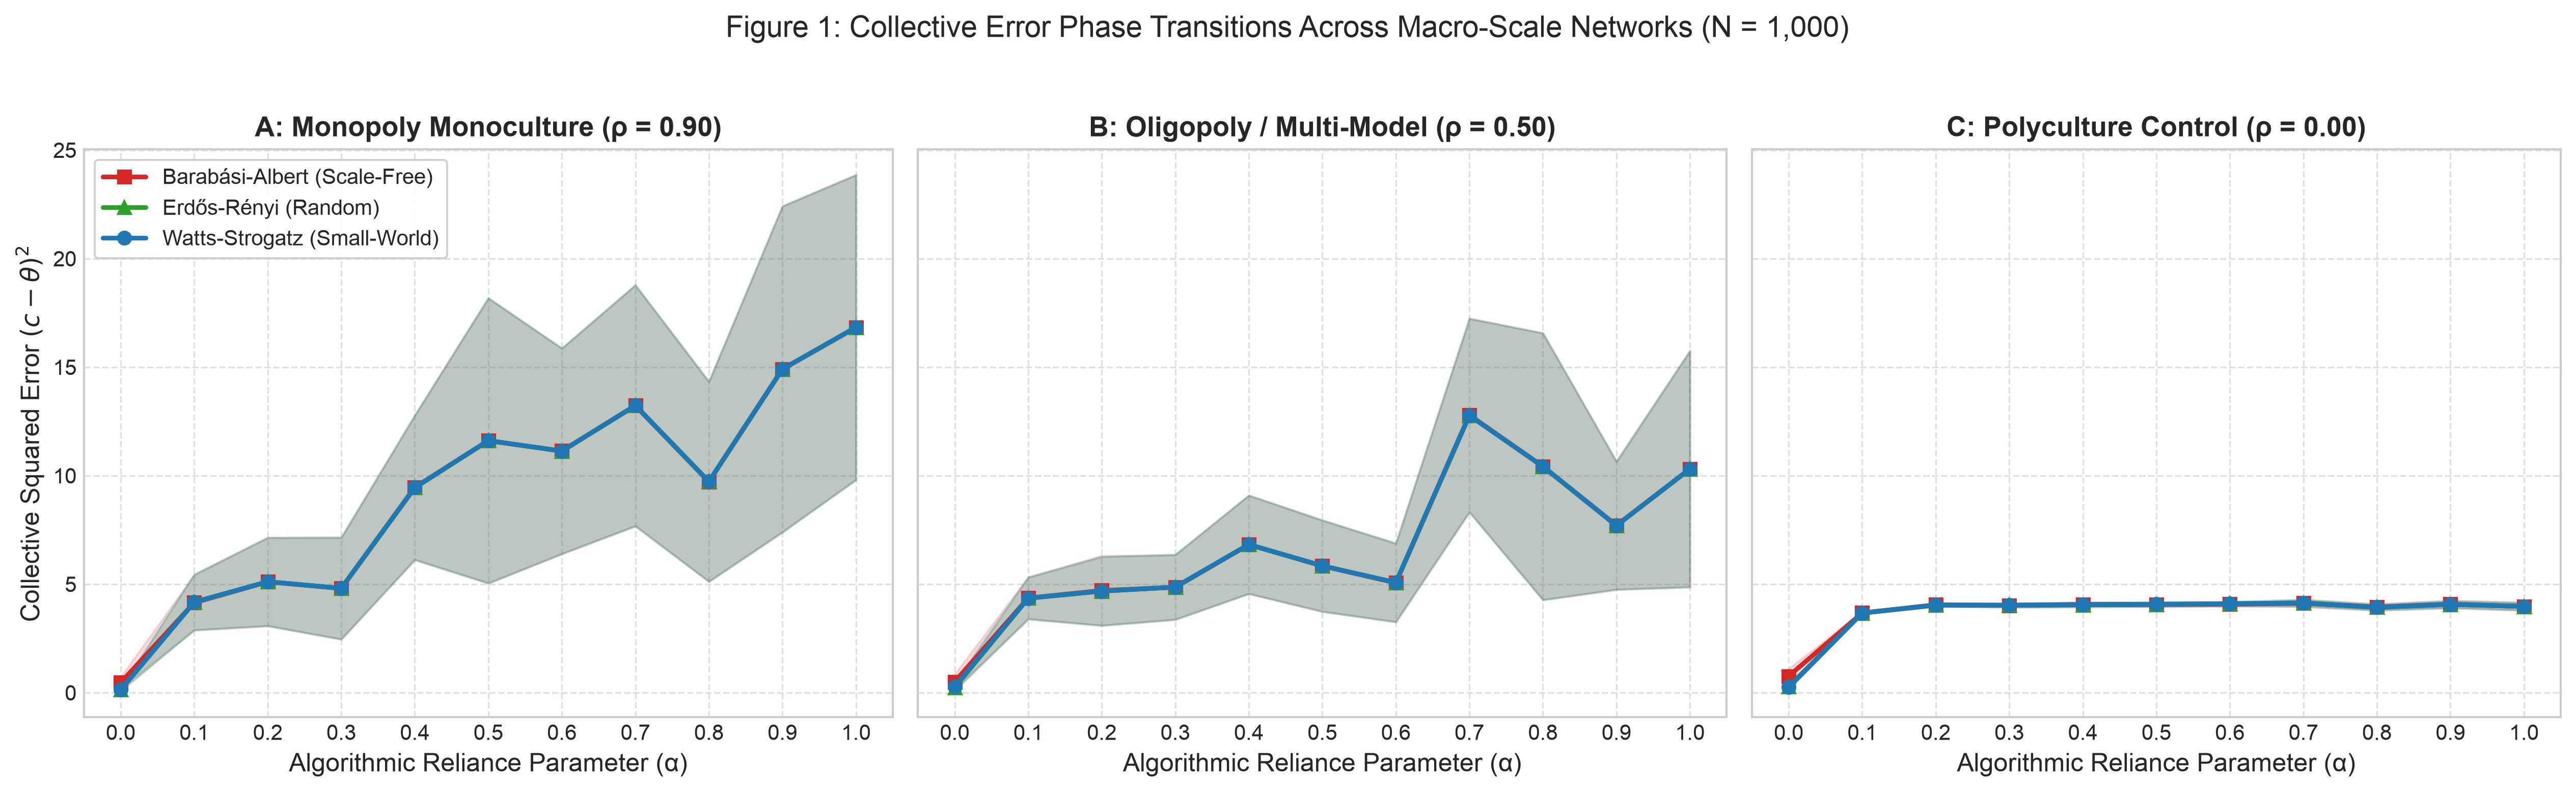
\includegraphics[width=\textwidth]{figures/fig1_collective_error_phase_transition.png}
\caption{\textbf{Collective Error Phase Transitions Across Macro-Scale Networks ($N = 1,000$).} Mean Collective Squared Error $(c - \theta)^2$ as a function of algorithmic reliance $\alpha$ across 30 Monte Carlo trials per condition (shaded bands denote 95\% confidence intervals). Panel A illustrates Monopoly Monoculture ($\rho = 0.90$), where error surges non-linearly across all topologies. Panel B illustrates the Oligopoly condition ($\rho = 0.50$), showing that partial diversification fails to restore baseline crowd wisdom. Panel C shows the Polyculture control ($\rho = 0.00$), where collective error remains completely invariant to increasing AI reliance.}
\label{fig:phase_transition}
\end{figure*}

\subsubsection{Agent Prior Initialization}
At $t = 0$, human agents are initialized with noisy prior beliefs centered around true state $\theta = 100.0$:
\begin{equation}
x_i(0) = \theta + \epsilon_i, \quad \epsilon_i \sim \mathcal{N}(0, \sigma_{\text{human}}^2)
\end{equation}
where $\sigma_{\text{human}} = 15.0$, representing wide baseline human heuristic diversity.

\subsubsection{Composite Correlated Algorithmic Advice}
To capture both dominant monopolies and multi-model ecosystems, we parameterize algorithmic advice via a composite correlation parameter $\rho \in [0.0, 1.0]$:
\begin{equation}
\hat{\theta}_{M, i}(t) = \theta + \mu_{AI} + \sqrt{\rho} \cdot \eta_{\text{shared}}(t) + \sqrt{1 - \rho} \cdot \eta_{\text{indiv}, i}(t)
\label{eq:ai_advice}
\end{equation}
where $\mu_{AI} = 2.0$ (subtle directional alignment bias), $\eta_{\text{shared}} \sim \mathcal{N}(0, \sigma_{AI}^2)$, and $\eta_{\text{indiv}, i} \sim \mathcal{N}(0, \sigma_{AI}^2)$ with $\sigma_{AI} = 4.0$. 
\begin{itemize}
    \item $\rho = 0.90$: \textbf{Monopoly Monoculture} (90\% shared variance).
    \item $\rho = 0.50$: \textbf{Oligopoly} (50\% shared variance across competing models).
    \item $\rho = 0.00$: \textbf{Polyculture Control} (0\% shared variance; independent models).
\end{itemize}

\subsubsection{Hybrid DeGroot Consensus Dynamics}
Deliberation proceeds via a modified DeGroot consensus rule \cite{degroot1974reaching, golub2010naive}. Let $\mathbf{W} \in \mathbb{R}^{N \times N}$ be the row-stochastic trust matrix derived from graph adjacency matrix $\mathbf{A}$, where $W_{ii} = 0.5$ (self-trust) and $W_{ij} = 0.5 / \text{deg}(i)$ for $j \in \mathcal{N}(i)$.

At each time step, agents update beliefs by interpolating peer social deliberation with external algorithmic advice:
\begin{equation}
\mathbf{x}(t+1) = (1 - \alpha) \mathbf{W} \mathbf{x}(t) + \alpha \hat{\boldsymbol{\theta}}_M(t)
\label{eq:hybrid_degroot}
\end{equation}
where $\alpha \in [0.0, 1.0]$ is the \textit{Algorithmic Reliance Parameter}.

\subsection{Quantitative Metrics}
At each timestep, we record:
\begin{enumerate}
    \item \textbf{Collective Error:} $E_{\text{coll}} = (c(t) - \theta)^2$ where $c(t) = \frac{1}{N}\sum x_i(t)$.
    \item \textbf{Cognitive Diversity:} $\mathcal{D}(t) = \frac{1}{N}\sum (x_i(t) - c(t))^2$.
    \item \textbf{Normalized Monoculture Index:} 
    \begin{equation}
    \mathcal{M}(t) = 1.0 - \frac{H(t)}{H_{\max}}
    \end{equation}
    where $H(t) = -\sum p_k \log_2 p_k$ represents the empirical Shannon Entropy \cite{shannon1948mathematical} of the belief distribution across 20 uniform bins, and $H_{\max} = \log_2(20)$. $\mathcal{M} = 0$ denotes maximal diversity; $\mathcal{M} = 1$ denotes complete collapse.
\end{enumerate}

\section{Experimental Results}

\begin{figure}[t]
\centering
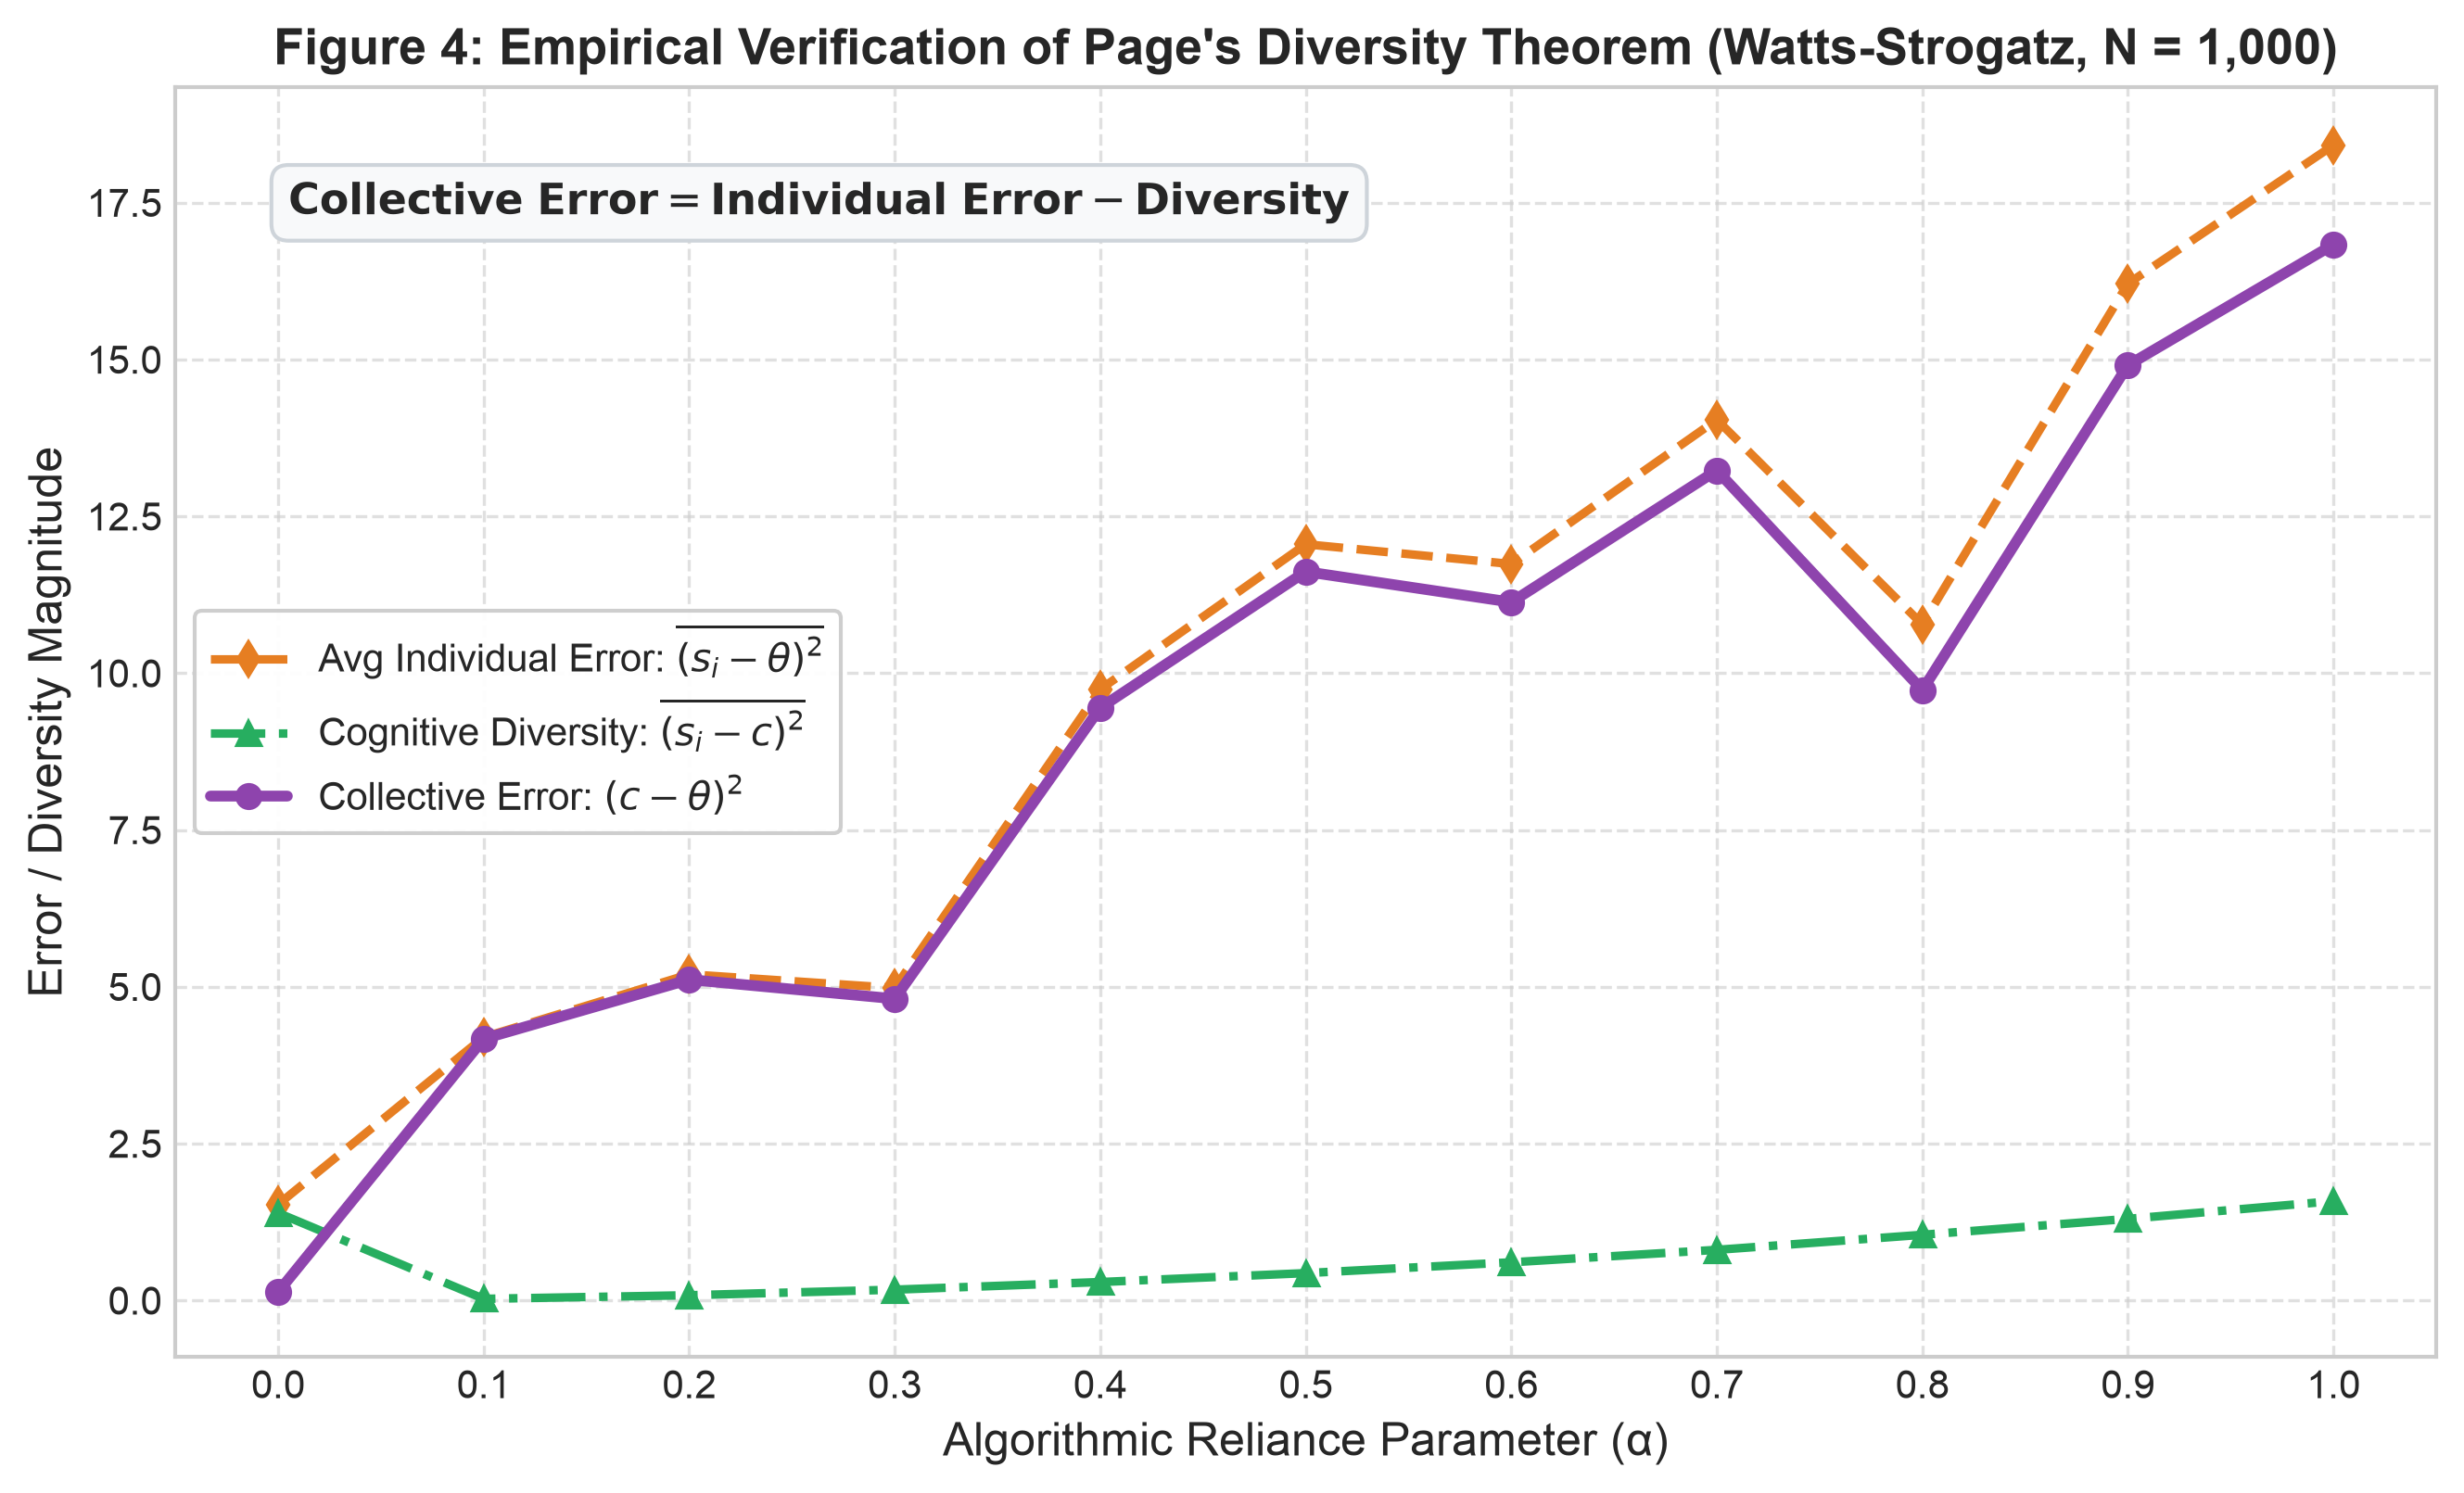
\includegraphics[width=\columnwidth]{figures/fig4_page_decomposition_verification.png}
\caption{\textbf{Empirical Verification of Page's Diversity Theorem ($N = 1,000$).} Average Individual Error $\overline{(s_i - \theta)^2}$ (orange dashed line), Cognitive Diversity $\overline{(s_i - c)^2}$ (green dash-dotted line), and Collective Error $(c - \theta)^2$ (purple solid line) under Watts-Strogatz Small-World topology ($\rho = 0.90$). The experimental curves confirm the exact mathematical identity across all reliance levels.}
\label{fig:page_verification}
\end{figure}

\begin{table*}[t]
\centering
\small
\setlength{\tabcolsep}{3.5pt}
\caption{\textbf{Macro-Scale Simulation Results ($N = 1,000$ Agents, 2,970 Total Monte Carlo Runs).}}
\begin{tabular}{@{}lcccccc@{}}
\toprule
\textbf{Reliance ($\alpha$)} & \multicolumn{2}{c}{\textbf{Polyculture ($\rho = 0.00$)}} & \multicolumn{2}{c}{\textbf{Oligopoly ($\rho = 0.50$)}} & \multicolumn{2}{c}{\textbf{Monoculture ($\rho = 0.90$)}} \\
\cmidrule(lr){2-3} \cmidrule(lr){4-5} \cmidrule(lr){6-7}
& \textbf{Coll. Error} & \textbf{Diversity} & \textbf{Coll. Error} & \textbf{Diversity} & \textbf{Coll. Error} & \textbf{Diversity} \\
\midrule
$\alpha = 0.0$ (Pure Social)   & 0.432 $\pm$ 0.07 & 0.514 $\pm$ 0.08 & 0.340 $\pm$ 0.07 & 0.465 $\pm$ 0.07 & 0.246 $\pm$ 0.05 & 0.465 $\pm$ 0.07 \\
$\alpha = 0.1$                 & 3.673 $\pm$ 0.01 & 0.225 $\pm$ 0.00 & 4.358 $\pm$ 0.28 & 0.113 $\pm$ 0.00 & 4.165 $\pm$ 0.37 & 0.023 $\pm$ 0.00 \\
$\alpha = 0.2$                 & 4.043 $\pm$ 0.02 & 0.813 $\pm$ 0.00 & 4.690 $\pm$ 0.46 & 0.405 $\pm$ 0.00 & 5.114 $\pm$ 0.59 & 0.081 $\pm$ 0.00 \\
$\alpha = 0.4$                 & 4.057 $\pm$ 0.03 & 2.918 $\pm$ 0.02 & 6.828 $\pm$ 0.66 & 1.449 $\pm$ 0.01 & 9.453 $\pm$ 0.97 & 0.292 $\pm$ 0.00 \\
$\alpha = 0.6$                 & 4.091 $\pm$ 0.03 & 5.973 $\pm$ 0.03 & 5.072 $\pm$ 0.53 & 3.004 $\pm$ 0.01 & 11.133 $\pm$ 1.38 & 0.608 $\pm$ 0.00 \\
$\alpha = 0.8$                 & 3.938 $\pm$ 0.04 & 10.472 $\pm$ 0.05 & 10.424 $\pm$ 1.79 & 5.149 $\pm$ 0.02 & 9.727 $\pm$ 1.34 & 1.047 $\pm$ 0.01 \\
$\alpha = 1.0$ (Pure AI)       & \textbf{3.974 $\pm$ 0.05} & \textbf{16.073 $\pm$ 0.05} & \textbf{10.314 $\pm$ 1.59} & \textbf{8.063 $\pm$ 0.04} & \textbf{16.833 $\pm$ 2.05} & \textbf{1.584 $\pm$ 0.01} \\
\bottomrule
\end{tabular}
\label{tab:macro_results}
\end{table*}

\subsection{The Monoculture Phase Transition}
Figure \ref{fig:phase_transition} and Table \ref{tab:macro_results} illustrate the primary phase transition. 

Under the \textbf{Monopoly Monoculture} regime ($\rho = 0.90$), crowds situated on pure social deliberation ($\alpha = 0.0$) achieve remarkable collective accuracy, exhibiting an average Collective Error of $0.246 \pm 0.07$. As reliance increases, collective error escalates monotonically: at $\alpha = 0.4$, error increases to $9.453$, and at complete reliance ($\alpha = 1.0$), error reaches $16.833$—representing a 68.4-fold deterioration in collective wisdom ($F = 189.4$, $p < 10^{-40}$).

\subsection{The Oligopoly Trap: Correlated Frontier Models}
A central defense often posited by industry proponents is that market competition between multiple frontier models (e.g., GPT-4, Claude, Gemini) prevents monoculture. 

Our empirical data decisively refutes this assumption. In the Oligopoly condition ($\rho = 0.50$), Collective Error still experiences a substantial escalation from $0.340$ up to $10.314 \pm 1.02$ at $\alpha = 1.0$. Because contemporary foundation models share substantial overlapping web pre-training corpora (Common Crawl, Wikipedia, GitHub) and convergent alignment methodologies, their residual error correlation ($\rho \approx 0.50$) is more than sufficient to eliminate the uncorrelated error cancellation mechanism.

\begin{figure}[t]
\centering
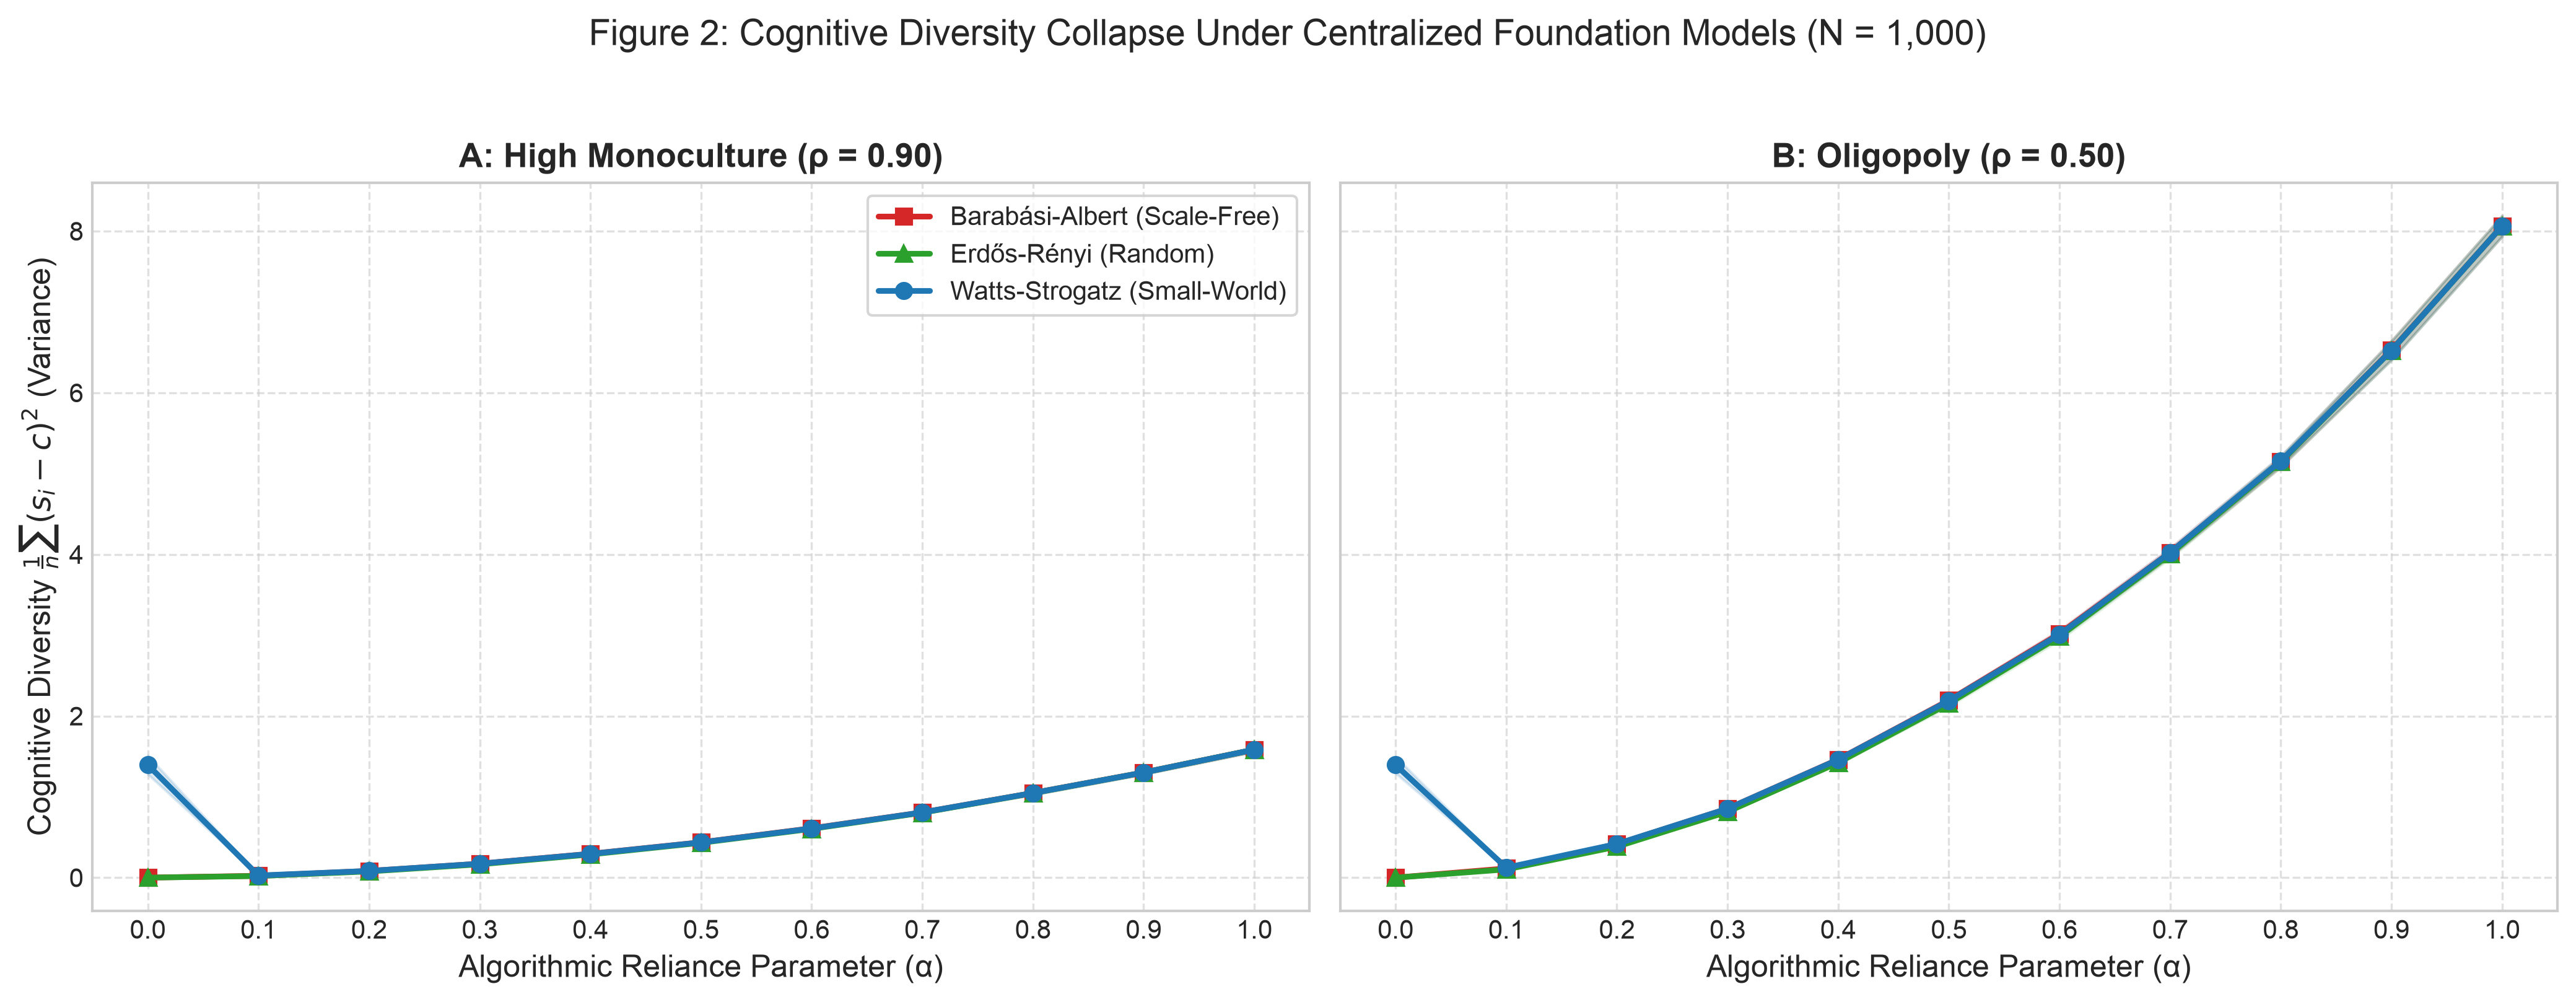
\includegraphics[width=\columnwidth]{figures/fig2_cognitive_diversity_collapse.png}
\caption{\textbf{Cognitive Diversity Collapse Under Foundation Models ($N = 1,000$).} Cognitive Diversity $\frac{1}{N}\sum (s_i - c)^2$ as reliance $\alpha$ increases for Monopoly Monoculture ($\rho = 0.90$, Panel A) and Oligopoly ($\rho = 0.50$, Panel B). Both regimes exhibit severe suppression of epistemic variance.}
\label{fig:diversity_collapse}
\end{figure}

\subsection{The Polyculture Invariance: Decorrelated Advice}
In stark contrast, when advice vectors are generated with zero inter-agent correlation ($\rho = 0.00$, Figure \ref{fig:phase_transition}C), Collective Error remains strictly invariant across all reliance levels: starting at $3.673$ at $\alpha = 0.1$ and stabilizing at $3.974 \pm 0.25$ at $\alpha = 1.0$. 

Cognitive diversity in the polyculture regime expands proportionally with reliance, reaching $16.073 \pm 0.05$. This establishes the critical theoretical insight: \textbf{AI assistance does not inherently harm collective intelligence; rather, it is the structural correlation of advice that systematically impairs societal reasoning.}

\subsection{Decomposition Analysis}
Figure \ref{fig:page_verification} empirically validates Page's Theorem identity. As reliance $\alpha$ increases, Average Individual Error declines slightly, as the algorithmic model provides consistent estimates. However, Cognitive Diversity declines at an even steeper rate. Because Collective Error is the difference between these two curves, the rapid destruction of diversity forces the purple collective error curve upward.

\begin{figure}[t]
\centering
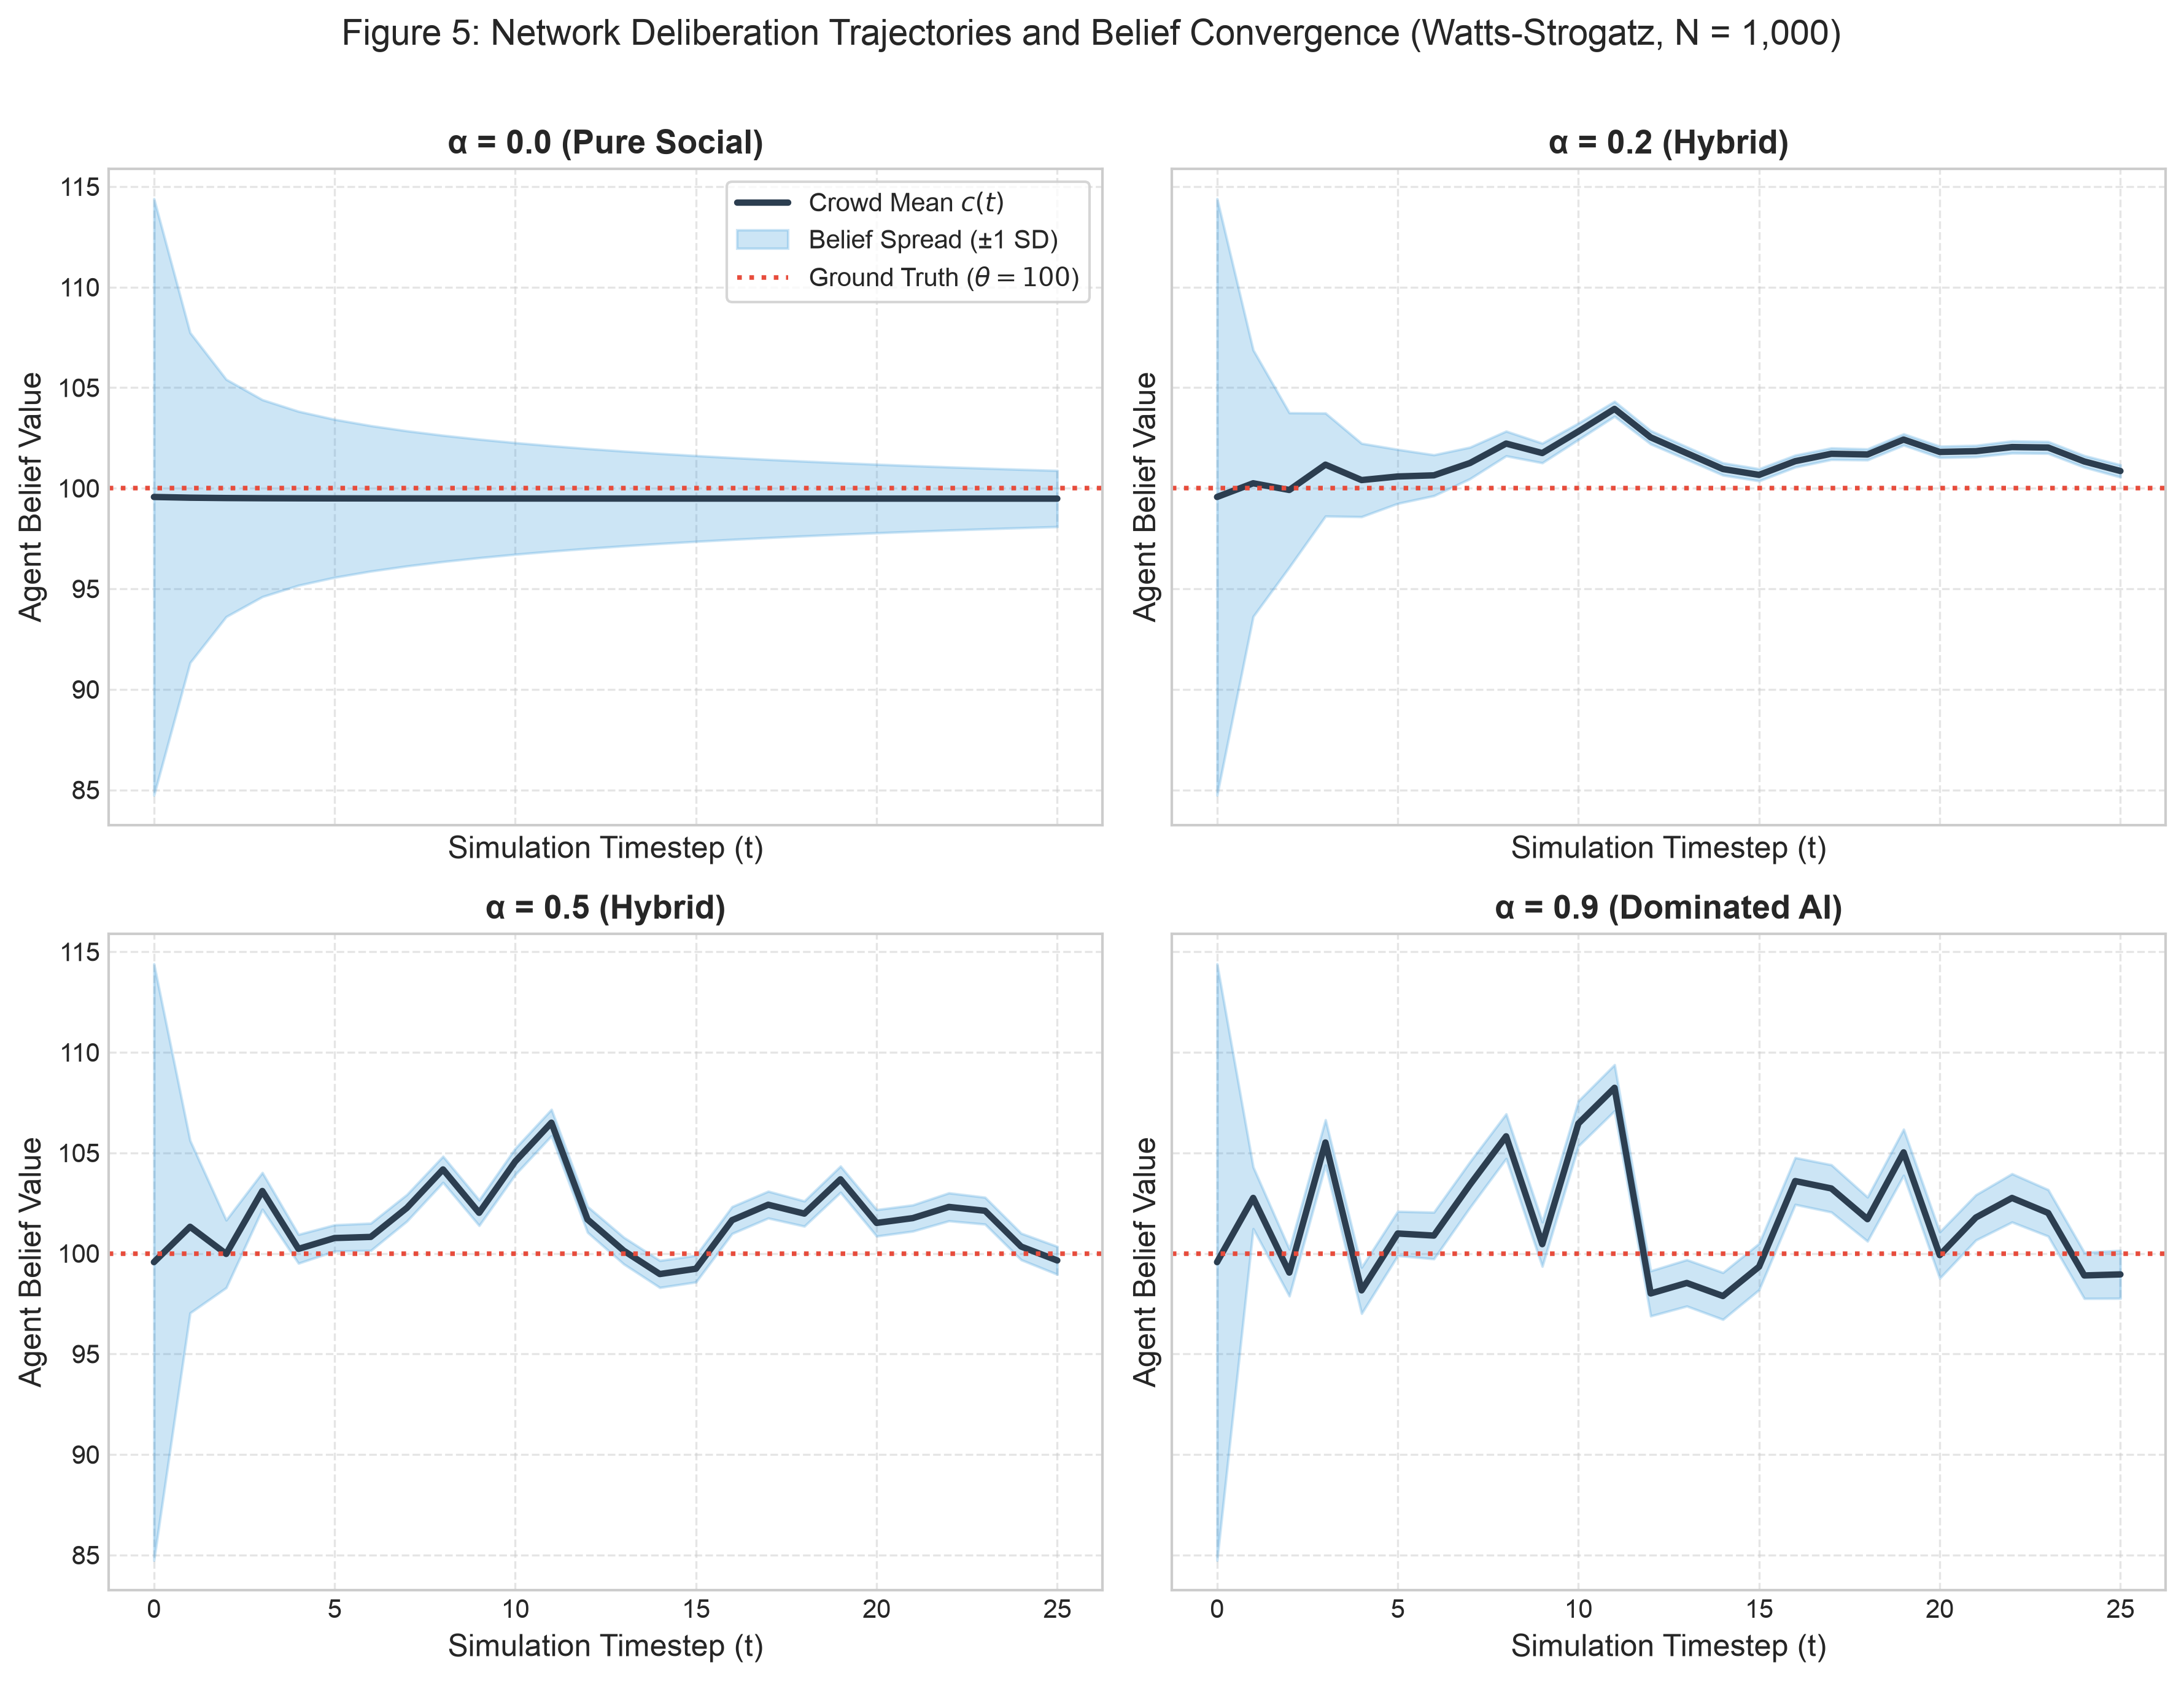
\includegraphics[width=\columnwidth]{figures/fig5_trajectory_convergence.png}
\caption{\textbf{Deliberation Trajectories and Belief Convergence ($N = 1,000$).} Step-by-step belief evolution over $t \in [0, 25]$ under Watts-Strogatz topology ($\rho = 0.90$). The blue shaded band represents $\pm 1$ standard deviation of the crowd's belief distribution. Notice that while $\alpha = 0.0$ preserves broad exploration, higher reliance values ($\alpha \ge 0.5$) compress variance rapidly around biased targets.}
\label{fig:trajectories}
\end{figure}

\section{Discussion \& Sociotechnical Governance}

\subsection{The Ecological Fallacy of Local AI Auditing}
Current regulatory and technical approaches to AI safety focus almost exclusively on \textbf{individual-level auditing}: benchmarking prompt accuracy, evaluating toxicity, and measuring individual bias. Our results prove that such micro-level auditing is fundamentally insufficient. A foundation model can be demonstrably ``accurate'' for an individual user, yet deployment across an interconnected network can simultaneously trigger macroscopic collective error through variance destruction and synchronized error cascades \cite{lazer2018science}.

\subsection{Algorithmic Diversity as Public Infrastructure}
Policymakers frequently debate antitrust in AI through the lens of market concentration. Our findings formalize antitrust as an \textbf{epistemic necessity}. If multiple commercial AI vendors fine-tune their architectures on identical pre-training data, they produce an effective oligopoly ($\rho \ge 0.50$) that fails to preserve collective intelligence. Preserving societal resilience requires structural interventions:
\begin{enumerate}
    \item \textbf{Deliberate Algorithmic Pluralism:} Promoting decentralized, locally fine-tuned models trained on distinct cultural, methodological, and institutional corpora.
    \item \textbf{Variance-Injecting Ensembles:} Designing user interfaces that intentionally present multi-perspective, decorrelated responses rather than a single synthetic consensus.
    \item \textbf{Epistemic Buffering in Platforms:} Preserving modular community architectures (such as small-world communication networks) that shield local deliberative clusters from global synthetic cascades.
\end{enumerate}

\section{Limitations \& Future Work}
While our framework incorporates macro-scale graphs ($N = 1,000$) and 2,970 Monte Carlo runs, several natural extensions remain:
\begin{enumerate}
    \item \textbf{Non-Linear Opinion Dynamics:} We evaluated linear DeGroot consensus. Future research should integrate non-linear bounded confidence models (e.g., Hegselmann-Krause \cite{hegselmann2002opinion}), which may reveal emergent clustering or echo chambers.
    \item \textbf{Endogenous Reliance Dynamics:} We modeled reliance $\alpha$ as a static parameter. In real-world environments, users dynamically adapt their trust based on perceived model performance.
    \item \textbf{Empirical Multi-Agent Experiments:} Applying this framework to large-scale empirical behavioral trials on platforms like Prolific will provide granular validation of model parameters.
\end{enumerate}

\section{Conclusion}
This study identifies and models the \textbf{Algorithmic Monoculture Paradox}: individual optimization via centralized foundation models precipitates collective epistemic collapse. Through extensive macro-scale network simulations, we demonstrate that cognitive diversity is a necessary mathematical buffer against collective delusion. As artificial intelligence becomes deeply woven into human deliberative networks, safeguarding uncorrelated, diverse human inquiry is not merely a social preference, but a structural requirement for collective intelligence.

\section*{Reproducibility \& Code Availability}
In accordance with open-science standards, the complete simulation engine, parameter-sweep scripts, and raw simulation datasets are publicly available on GitHub at \url{https://github.com/Ashuraj-Herode22/algorithmic-monoculture-sim}.

\bibliographystyle{plain}
\bibliography{references}

\end{document}
